%%%%%%%%%%%%%%%%%%%%%%%%%%%%%%%%%%%%%%%%%%%%%%%%%%%%%%%%%%%%%%%%%%%%%%%%%%%%%%%%%%%%%%%%%%%%%%%%%%%%%%%%
%%%%%%%%%%%%%%%%%%%%%%%%%%%%%%%%%%%%%%%%%%%%%%%%%%%%%%%%%%%%%%%%%%%%%%%%%%%%%%%%%%%%%%%%%%%%%%%%%%%%%%%%
											   % Structural Estimation
%%%%%%%%%%%%%%%%%%%%%%%%%%%%%%%%%%%%%%%%%%%%%%%%%%%%%%%%%%%%%%%%%%%%%%%%%%%%%%%%%%%%%%%%%%%%%%%%%%%%%%%%
%%%%%%%%%%%%%%%%%%%%%%%%%%%%%%%%%%%%%%%%%%%%%%%%%%%%%%%%%%%%%%%%%%%%%%%%%%%%%%%%%%%%%%%%%%%%%%%%%%%%%%%%
\section{Structural Estimation}\label{sec:struc_est}
The expressions to compute the terms capturing taste and choice set differences crucially depend on the product variety- and firm-level elasticities of substitution. This section starts with estimating the product variety level elasticities of substitution and uses these estimates to construct firm-level price and quantity indices used to estimate the firm-level elasticities of substitution. In turn, we use these elasticities of substitution to construct cost-of-living differences and provide a first look into the size of cost-of-living differences and the importance of the three terms of the decomposition. 

\subsection{Elasticities of Substitution}
\subsubsection{Product variety-level elasticities - $\sigma_p$}
\paragraph{Estimation strategy}
To estimate the variety-level elasticity of substitution, we return to the product variety-level demand system. Demand for product variety $i$ in region $l$ at time $t$ is given by: 
\begin{linenomath*}
    \begin{equation*}
        C_{il,t} = \varphi_{il,t}^{\sigma_p-1}\left(\frac{P_{il,t}}{P_{fpl,t}}\right)^{-\sigma_p}C_{fpl,t}  
    \end{equation*}
\end{linenomath*}
\noindent as before $C_{il,t}$ is the consumed quantity in terms of metric units, $\varphi_{il,t}$ is the taste parameter and $P_{il,t}$ is the unit price for product variety $i$ in region $l$ at time $t$. In addition, $P_{fpl,t}$ and $C_{fpl,t}$ are the firm-level price index and consumption index in region $l$ at time $t$ and $\sigma_p$ is the product variety-level elasticity of substitution. Taking logs, we have: 
\begin{linenomath*}
    \begin{equation*}
        c_{il,t} = - \sigma_p p_{il,t} + \sigma_p p_{fpl,t} + c_{fpl,t} + (\sigma_p-1)\text{ln}\left(\varphi_{il,t}\right)
    \end{equation*} 
\end{linenomath*}
\noindent where small letters indicate logarithmic transformations of the level variables, e.g. $c_{il,t} \equiv \text{ln}\left(C_{il,t}\right)$. To estimate elasticities of substitution, we rely on the fact that after collapsing the household dimension in the transaction data the unit of observation is at the product variety-region-retail chain-time level. In practice, we consider the following model: 
\begin{linenomath*}
    \begin{equation}\label{eq:struc_est_elas_bar}
        c_{icl,t} = - \sigma_{p} p_{icl,t} + \theta_{icn(l),y(t)} + \theta_{icn(l),w(t)} + \lambda_{fpcl,t} + \varepsilon_{icl,t}
    \end{equation}
\end{linenomath*}
\noindent where $\varepsilon_{icl,t}$ subsumes the structural residual $\varphi_{il,t}$. Estimating the elasticities of substitution is subject to two endogeneity concerns. First, the price and consumption index $P_{fpl,t}$ and $C_{fpl,t}$ depend on the structural residuals that determine the quantity level. Second, if price variation is due to temporary discounts and promotions, product variety-level prices are likely correlated with the structural residual as well. We deal with the first issue by including firm-category-chain-NUTS2-time fixed effects $\lambda_{fpcl,t}$. The inclusion of a full set of fixed effects at the level of the indices is a common strategy to soak up this variation (e.g. \citet{Atkin2018, Fajgelbaum2020}). Moreover, the addition of $\lambda_{fpcl,t}$ also controls for any time-varying region-chain-specific demand shock that affects the product varieties of a specific firm in the same way. Collapsing the data at the variety-region-chain-time dimension is important to deal with the second identification concern. \citet{Dellavigna2019} illustrates that retail chains tend to follow uniform pricing strategies in which they frequently change prices over time through temporary discounts while limiting spatial variation to a minimum.\footnote{\citet{Dellavigna2019} point to managerial inertia, agency costs and threats to brand image as possible explanations for why retail chains adopt (potentially suboptimal) uniform pricing strategy.} The idea behind the identification strategy is that once we condition on the seasonal variation in prices and quantities, the lower-frequency variation in prices and quantities should reflect variation due to cost factors. To this end, we include highly-detailed product variety-chain-country-year fixed effects, $\theta_{icn(l),y(t)}$, and product variety-chain-country-week-of-the-year fixed effects, $\theta_{icn(l),w(t)}$. By interacting product variety-retail chain-country fixed effects with week-of-the-year and year effects, we capture seasonal variation in prices and quantities across variety-store cells at the weekly frequency and allow this pattern to shift across the years. However, even conditional on these fixed effects, there might still be price variation that is potentially correlated with occasional local demand shocks outside of this recurring seasonal pattern at the country level. Therefore, we instrument product variety-chain level prices with the average within-chain product variety level price across the other regions. The suitability of this \citet{Hausman1996}-type instrument relies on the exclusion restriction that chain-level pricing strategies are assumed not to be correlated anymore with local demand shocks after conditioning on the seasonal pattern of promotions and discounts.\footnote{In the estimation, we rely on the following moment condition $\mathbb{E}_{t}\left[{\varepsilon_{icl,t}|\bar{p}_{ic-l,t},\boldsymbol{\theta},\boldsymbol{\lambda}}\right] = 0$ and minimize the following GMM-objective function to obtain: 
\begin{equation*}
    \widehat{\sigma_p} = \argmin_{\sigma_p} \boldsymbol{M}(\sigma_p)'\boldsymbol{W}\boldsymbol{M}(\sigma_p) \qquad \forall p \in \mathcal{P} 
\end{equation*}
where 
\begin{equation*}
    M_{icl}(\sigma_p) = \mathbb{E}_{t}\left[\bar{p}_{ic-l,t}\varepsilon_{icl,t}(\sigma_p)\right], \qquad 
    \bar{p}_{ic-l,t} \equiv \frac{1}{N_{lc}} \sum_{k \in \mathcal{L}_c\setminus l} p_{ick,t}  
\end{equation*}
and $\boldsymbol{W}$ is a weighting matrix that weights the product variety-region moment conditions using the number of transactions associated with that product variety in that region. For this reason, our estimator is very similar to the one developed in \citet{Dellavigna2019} but different from \citet{Faber2021} which estimates brand-level elasticities in the US using only regional variation and no variation across retail chains and different from \citet{Atkin2018} which use it to estimate store-level elasticities in Mexico by collapsing the product variety dimension.}

\paragraph{Baseline results}    We estimate the elasticities using data at the product variety-retail chain-NUTS2-week level. We restrict the sample by placing restrictions on the frequency by which product varieties appear with positive sales. This is because there is widespread evidence of the existence of many zeros in scanner data which might potentially downwardly bias the elasticity estimates (e.g. \citet{Dube2021, Gandhi2022}). Given our broad focus on many product categories, it is hard to obtain exogenous variation in choice set determination for each product category as in \citet{Dube2021}. Instead, we choose to only include product varieties that are frequently purchased and thus suffer less from zero market shares. Below, we discuss the sensitivity of the estimates to alternative sample restrictions. Figure \ref{fig: app_elas_sigma_cats_weekly_50ptt} and Table \ref{tab: app_elas_sigma_cats_weekly} present the baseline OLS and IV estimates and report clustered standard errors at the product variety level. As expected, all OLS estimates have a negative sign and are precisely estimated but also represent quite inelastic residual demand curves. Their distribution is centered around $-1.02$ and has a 10\%-90\% spread of $[-1.96,-0.22]$. As the OLS estimates may still suffer from the simultaneous determination of prices and quantities, we instrument prices with the Hausman-type instrument. Figure \ref{fig: app_elas_sigma_cats_weekly_50ptt} shows that the IV-estimates are quite precisely estimated.\footnote{The precision of the IV-estimates is due to the generally high first-stage F-statistics. The Kleibergen-Paap statistic has an unreported 10\%-90\% range of $[12.35, 1098.44]$ across product categories.} In addition, they are almost always more negative compared to the OLS estimates. The IV estimates have a 10\%-90\% spread of $[-4.77,-1.15]$ with a median estimate of $-2.77$. While this product variety level estimates are more inelastic than the ones reported in \citet{Hottman2016}, the estimates are quantitatively in line with the estimates reported in different strands of literature. For instance, \citet{Dellavigna2019}, \citet{Faber2021} and \citet{Dopper2022} (for comparable US scanner data) and \citet{Fajgelbaum2020} (for US trade data at the product variety level) estimate very similar median estimates.\footnote{These papers report median elasticities of -2.6, -2.2, slightly below -2 and -2.53 respectively} In addition, we reject the null hypothesis that the elasticities are equal to the theoretical constraint of $-1$ for all but two product categories.\footnote{Unfortunately, we are unable to estimate elasticities of substitution for the Skincare - Makeup and Infant food categories because they have too few observations, conditional on the fixed effects. However, failing to obtain IV-estimates is common (see e.g. \citet{Hottman2016, Jaravel2019}) and we explain in section \ref{sec:border_effects_eu} how we deal with this to obtain the structural components.} Nevertheless, when estimating cost-of-living differences we experiment with more elastic elasticities of substitution that are closer to the ones from \citet{Hottman2016} and show that qualitative conclusions are robust.

\paragraph{Robustness}      We consider three different robustness checks. First, the baseline results are obtained by placing restrictions on how frequently positive sales are observed across weeks in a given year. Table \ref{tab: app_elas_sigma_cats_weekly} shows that the IV estimates are less elastic when we do not place any restrictions on the sample. In this case, the distribution of IV estimates has a 10\%-90\% range of $[-3.45,0.52]$. By placing ever stricter restrictions on the sample in terms of the frequency of positive sales and on the actual importance of different product varieties, the elasticity estimates become more elastic. When we restrict the frequency at 26 weeks and the product variety-level market share at 0.1\%, the distribution of elasticities is almost identical. Hence, we view the restriction on the frequency of more than or equal to 50\% as striking a good balance. Second, the baseline specification uses data at the weekly frequency. Figure \ref{fig: app_elas_sigma_cats_monthly_50ptt} and Table \ref{tab: app_elas_sigma_cats_monthly} shows the results when we estimate the elasticities using monthly data. The monthly IV estimates are almost always precisely estimated but they are also generally more inelastic. In addition, Table \ref{tab: app_elas_sigma_cats_monthly} indicates that there are slightly more product categories for which the theoretical constraint is not satisfied. For this reason, we stick with the weekly estimates as input for the subsequent analyses. Finally, the theoretical framework does not have a retail chain dimension and therefore there is some leeway as to how we deal with regional time-varying demand shocks. Table \ref{tab: app_elas_sigma_cats_weekly} provides an overview of the results when we experiment with alternative fixed effects. When we replace the firm-chain-category-region-time fixed effects with firm-chain-category-country-time fixed effects, we recover a more elastic median demand elasticity of $-3.89$, but also with a much wider range of $[-8.89;4.20]$.\footnote{One potential explanation for the more elastic demand estimates when including time-varying fixed effects at the country level is that if promotional activities come with temporary price reductions and if there is regional variation in promotional activity, only including time-varying fixed effects at the country level will overestimate the elasticity of demand. This is because in this case the increase in consumption and the fall in the price are both driven by the same promotion. As $\sigma_{c,prom} > 0$ and  $\sigma_{p,prom} < 0$ the elasticity of substitution would be downward biased.} In addition, the number of product categories where the theoretical restriction is not satisfied rises from 2 to 10. When we only include firm-category-region-time fixed effects instead of the firm-chain-category-region-time fixed effects, the 10\%-90\% range is $[-5.01,-1.15]$ centered around $-3.12$. This specification also leads to more estimates that violate the theoretical constraint. The robustness exercise of cost-of-living differences to alternative elasticities includes the implied elasticities with country-level fixed effects and the results presented below are also robust to using alternative fixed effects in the estimation of the elasticities.

\subsubsection{Firm-level elasticities - $\eta_p$}
\paragraph{Estimation strategy}     To estimate the firm-level elasticities of substitution, consider the residual demand curve for firm $f$ in product category $p$ in region $l$ at time $t$: 
\begin{linenomath*}
    \begin{equation*}
        C_{fpl,t} = \varphi_{pfl,t}^{\eta_p-1}\left(\frac{P_{fpl,t}}{P_{pl,t}}\right)^{-\eta_p}C_{pl,t}  
    \end{equation*}
\end{linenomath*}
\noindent where $C_{pfl,t}$ and  $P_{fpl,t}$ are the firm-level quantity and price level, $P_{pl,t}$ and $C_{pl,t}$ are the aggregate price and consumption index and $\eta_p$ governs how consumers substitute across firms in product category $p$. $\varphi_{pfl,t}$ is the firm-level taste parameter that shifts demand across all product varieties in product category $p$ offered by firm $f$. At any level of aggregation, the utility functions are homogeneous of degree 1 in the taste parameters. Therefore, without an additional normalization, it is impossible to distinguish between the firm-level tastes $\phi_{fpl,t}$ and the aggregated product-variety level taste parameters within each product category-firm-region-time combination. For this reason, we follow \cite{Hottman2016} and make two useful normalizations regarding the taste parameters: 
\begin{linenomath*}
    \begin{equation*}
        \tilde{\varphi}_{fpl,t} 
            \equiv  \left(\prod_{i \in \mathcal{B}_{fpl,t}} \varphi_{il,t} \right)^{\frac{1}{N_{fpl,t}}}
            =       \left(\prod_{f \in \mathcal{F}_{fpl,t+1}} \varphi_{fpl,t+1} \right)^{\frac{1}{N_{fpl,t+1}}}
            \equiv \tilde{\varphi}_{pl,t+1}
    \end{equation*}
\end{linenomath*}
\noindent where $N_{fpl,t}$ is the number of product varieties that firm $f$ sells in product category $p$ in region $l$ at time $t$ and $N_{pl,t}$ is the associated number of firms. We normalize the product variety level taste parameters $\varphi_{il,t}$ such that the geometric mean of the product variety level taste parameters within each product category-firm-region-time does not change over time.\footnote{Note that this normalization is without loss of generality as any geometric aggregator would be suitable (see \cite{Redding2020}). In addition, this normalization is different from the normalization we performed in the derivation of the cost-of-living differences across regions in two ways. First, the previous normalization was about ruling out that pure changes in tastes at the firm or product variety level across regions can induce changes in cost-of-living differences. In this case, the normalization is about how the product variety- en firm-level shifters are related within each region and is based on the fact that the utility aggregators are homogeneous of degree 1 in the taste parameters. Second, this normalization is about the full set of product varieties offered in region $l$. The previous normalization only covers the set of product varieties that is common across the two regions.} In this way, we ensure that differences in firm-level consumption levels conditional on relative prices and aggregate consumption are captured by $\varphi_{pfl,t}$ and any shifts in product variety-level consumption levels conditional on relative prices and firm-level consumption levels is captured by the $\varphi_{il,t}$'s. Consider the log transformation of the firm-level residual demand curve: 
\begin{linenomath*}
    \begin{equation*}
        c_{fpl,t} = - \eta_p p_{fpl,t} + \eta_p p_{pl,t} + c_{pl,t} + (\eta_p-1)\text{ln}\left(\varphi_{pfl,t}\right)
    \end{equation*} 
\end{linenomath*}

\noindent and its empirical counterpart are given by: 

\begin{linenomath*}
    \begin{equation}\label{eq:struc_est_elas_firm}
        c_{pfl,t} = - \eta_{p} p_{pfl,t} + \theta_{pfl} + \lambda_{pl,t} + \varepsilon_{pfl,t}
    \end{equation}
\end{linenomath*}
\noindent where $\varepsilon_{pfl,t}$ subsumes $\varphi_{pfl,t}$. We take the following steps to estimate equation \ref{eq:struc_est_elas_firm}. First, we obtain the firm-level consumption and price indices by aggregating product variety-level quantity and price using the baseline product-variety level elasticities of substitution and the backed-out product variety-level taste parameters.\footnote{We back out the product variety level demand shifters using: $$\varphi_{il,t} =  \frac{P_{il,t}}{\tilde{P}_{fpl,t}}\left(\frac{S_{il,t}}{\tilde{S}_{fpl,t}}\right)^{\frac{1}{\sigma_p-1}}\tilde{\varphi}_{fpl,t}$$ where $\tilde{P}_{fpl,t} \equiv \left(\prod_{i \in \mathcal{B}_{fpl,t}} P_{il,t}\right)^{\frac{1}{N_{fpl,t}}}$ and $\tilde{S}_{fpl,t} \equiv \left(\prod_{i \in \mathcal{B}_{fpl,t}} S_{il,t}\right)^{\frac{1}{N_{fpl,t}}}$.} We include two sets of fixed effects to deal with omitted variables and use an instrument to construct moment conditions. First, including the product category-region-time fixed effects $\lambda_{pl,t}$ captures variation stemming from the unobserved product category-level price and consumption indices, given by $p_{pl,t}$ and $c_{pl,t}$ respectively. In addition, these fixed effects pick up time-varying regional demand shocks that affect all firms similarly in product category $p$ in region $l$. Second, $\theta_{pfl}$ are category-firm-region fixed effects and pick up persistent differences in firm-level tastes across regions, such as the unweighted average product variety-level taste parameters $\varphi_{pfl,t}$. As the local demand shocks might still drive both consumption and prices, we rely on an instrument that follows from the structure of the demand system and the normalization imposed on the average product variety-level demand shifters. In particular, the firm-level price index can be written as a product of two intuitive terms (see Appendix \ref{app:theory_residuals_instrument} and \citet{Hottman2016}): 
\begin{linenomath*}
    \begin{equation*}
        P_{fpl,t} = \tilde{P}_{fpl,t} 
                    \left(
                        \sum_{i \in \mathcal{B}_{fpl,t}} \frac{S_{il,t}}{\tilde{S}_{fpl,t}} \tilde{\varphi}_{fpl,t}^{\sigma_p-1}
                    \right)^{\frac{1}{1-\sigma_p}}
    \end{equation*}
\end{linenomath*}
\noindent The first part is the unweighted geometric average across product variety-level prices offered by firm $f$ in product category $p$, region $l$ at time $t$. When firms simultaneously set the average firm-level price and taste parameter, this first part is correlated with the firm-level taste shifter $\varphi_{pfl,t}$. The second part of this expression depends on the dispersion in product variety level market shares within each product category-firm-region-time cell. Intuitively, more dispersion in market shares, reflecting greater dispersion in taste-adjusted prices, leads to a fall in the geometric average and thus an increase in the sum of market shares relative to their geometric average. However, as this sum is raised to a negative power ($1-\sigma_p$) greater dispersion within product category-firm-region-time cells leads to a fall in the firm-level price index. As the relative within product category-firm-region-time market shares do not depend on the firm-level taste shifter and the unweighted geometric average across product varieties is partialled out with the inclusion of $\theta_{pfl}$, the second part is uncorrelated with the firm-level taste parameter and therefore a suitable instrument.\footnote{This instrument relies on the presence of multi-product firms and imperfect substitutability across product varieties which. When only one product is supplied, the dispersion in market share is zero. If product varieties are perfect substitutes ($\sigma_p \rightarrow \infty$), market shares are disconnected from taste-adjusted prices leading to no dispersion in market shares. In the estimation, we rely on the following moment condition $\mathbb{E}_{t}\left[{\varepsilon_{fpl,t}|p^{D}_{fpl,t},\boldsymbol{\theta},\boldsymbol{\lambda}}\right] = 0$ and minimize the following GMM-objective function to obtain: 
\begin{equation*}
    \widehat{\eta_p} = \argmin_{\eta_p} \boldsymbol{M}(\eta_p)'\boldsymbol{W}\boldsymbol{M}(\eta_p) \qquad \forall p \in \mathcal{P} 
\end{equation*}
where 
\begin{equation*}
    M_{pfl}(\eta_p) = \mathbb{E}_{t}\left[p^{D}_{fpl,t}\varepsilon_{fpl,t}(\eta)\right], \qquad 
    p^{D}_{fpl,t} \equiv 
        \frac{1}{1-\hat{\sigma}_p}
        \text{ln}\left(\sum_{i \in \mathcal{B}_{fpl,t}}\frac{S_{il,t}}{\tilde{S}_{fpl,t}} \tilde{\varphi}_{fpl,t}^{\hat{\sigma_p}-1}\right)
\end{equation*}
and $\boldsymbol{W}$ is a weighting matrix that weights the product variety-region moment conditions using the number of transactions associated with that firm in that region.}

\paragraph{Baseline results}    We estimate the elasticities using data at the firm-NUTS2-week level and restrict the baseline sample to include all purchases on product varieties that register positive sales in more than 50\% of the time within a year. We present the baseline in Figure \ref{fig: app_elas_eta_cats_weekly_50ptt} and report an overview of all specifications in Table \ref{tab: app_elas_eta_cats_weekly_q} with clustered standard errors at the firm level. The OLS estimates are all negative, precisely estimated and almost always fall within the $[-2,-1]$ range. Given that firm-level prices conditional on the fixed effects might still be correlated with the structural residual, we turn to the IV estimates. First, the instruments are strong as the F-statistics of the first-stage regressions are almost always larger than the conventional rejection levels for weak instruments.\footnote{More precisely, the first-stage Kleibergergen-Paap F-statistics have a 10\%-90\% range of $[15.60;5,830.67]$ while the smallest F-statistics is $7.24$.} Second, the IV estimates imply more elastic residual demand curves as they are centered around $-3.10$ and have a 10\%-90\% range of $[-4.84,-1.71]$.\footnote{The range of firm-level elasticities is very close to the range of product-variety level elasticities. Given that we do not impose any restriction on their relative magnitude, this does not pose a problem for our analysis per se.} This range is still lower, but comparatively closer to the estimates in \citet{Hottman2016} which estimate firm-level elasticities between $[-7.3,-2.6]$ centered around $-3.9$. The estimation routine successfully ends for all product categories and we reject the null hypothesis that the elasticities are different from the theoretical constraint of $-1$ for all the product categories.

\paragraph{Robustness} We consider four robustness checks. First, Table \ref{tab: app_elas_eta_cats_weekly_q} shows that the elasticities are very similar across different sample restrictions. The reason for this is that the data becomes much less sparse when collapsing both retail chain and product variety dimensions such that imposing the same sample restrictions does not result in markedly different samples. At this level of aggregation, it does not matter whether we consider the full sample or the frequent sample. Second, similar to the product-variety estimates, the distribution of monthly firm-level elasticities is shifted upwards when we collapse the data at the monthly level. While the elasticities are still precisely estimated, Table \ref{tab: app_elas_eta_cats_monthly_q} shows that the distribution of monthly estimates is centered around $-1.66$ with a range $[-3.20,-1.32]$. Third, the baseline estimation includes product category-firm-region fixed effects and thus only controls for persistent differences across firms within regions. However, if retail chains and firms coordinate on seasonal price changes and promotion, a better identification strategy could be to use time variation conditional on seasonal shocks. For this reason, we re-estimate equation \ref{eq:struc_est_elas_firm} by replacing the $\theta_{pfl}$ fixed effects with product category-firm-region-yer fixed effects, $\theta_{pfl,y(t)}$, and product category-firm-region fixed effects-week-of-the-year $\theta_{pfl,w(t)}$. This set of fixed effects also flexibly controls for seasonal demand shocks that could drive both firm-level demand and prices. Nevertheless, Table \ref{tab: app_elas_eta_cats_weekly_q} shows that the distribution of elasticities is largely unaffected.

\paragraph{Cross-country Heterogeneity} The assumption that elasticities of substitution are common across countries is necessary to exactly decompose cost-of-living differences across regions. To check the validity of this assumption for the firm-level elasticities of substitution, we estimate country-level elasticities of substitution by interacting the price variable in equation \ref{eq:struc_est_elas_firm} with country dummies. Tables \ref{tab: app_elas_eta_cats_weekly_q_BE} - \ref{tab: app_elas_eta_cats_weekly_q_DE} present the elasticity of substitution estimates at the country level and Table \ref{tab: app_elas_eta_cats_weekly_q_comp} provides a comparison of the distribution of the IV-estimates across the different countries. Tables \ref{tab: app_elas_eta_cats_weekly_q_BE} - \ref{tab: app_elas_eta_cats_weekly_q_DE} confirm that the elasticities are still precisely estimated and satisfy the theoretical constraint in almost all cases. Even though there is some variation across countries for a couple of product categories, Table \ref{tab: app_elas_eta_cats_weekly_q_comp} shows that these differences do not imply large systematic differences in the country-level distributions. Therefore, the assumption of equal elasticities does not seem to be very restrictive.

\paragraph{Implied markups}    An additional check on the estimated elasticities of substitution is to see whether they imply firm-level markups when combined with an assumption on how firms set prices. If we assume that firms set prices in a simultaneous move Bertrand game, firm-level markups depend on the firm-level elasticity of substitution and on the firm-level market share in location $l$ at time $t$.\footnote{In particular, under Bertrand competition in prices, markups are given by: 
    \begin{equation}\label{eq:pricing_rule}
        P_{il,t} = \frac{\varepsilon_{fnp,t}}{\varepsilon_{fnp,t} - 1}MC_{il,t},
        \qquad \text{where} \qquad
        \varepsilon_{fnp,t} \equiv \eta_p - \left(\eta_p - 1 \right)S_{fpn,t} 
    \end{equation}} 
Figure \ref{fig: struct_est_markups} shows the full distribution of recovered firm-level markups across product category-firm-country-year observations. We recover a median firm-level markup of 1.5 which implies that the median firm charges a 50\% price premium over its marginal costs.

How sensible are these markup estimates? Because there is little empirical evidence on the level of firm-level markups for a comparable set of product categories in Europe, we benchmark our estimates to the broader literature on markup estimation. There are two broad strands in this literature. First, the demand approach estimates markups by specifying a model of demand and market structure. Markups are computed based on the estimated demand parameters and the optimal markup function as implied by the assumed market structure. Our approach falls in this strand. Other papers that take the demand approach to estimate markups for a broad set of product categories are \citet{Hottman2016} and \citet{Dopper2022}. While \citet{Hottman2016} finds a median markup of 1.31, \citet{Dopper2022} reports a median markup of 2.08.\footnote{These papers report different measures of the markup. \citet{Hottman2016} report a median $\frac{P-MC}{MC}$ of 0.31, which results in a median $\frac{P}{MC}$ of 1.31. \citet{Dopper2022} report a median Lerner index $\frac{P-MC}{P}$ of 0.48 which results in a median $\frac{P}{MC}$ of 2.08.} Second, \citet{Deloecker2012} pioneered the production approach in which the combination of cost minimization and an estimated output elasticity on a completely variable input in production yields markup estimates. \citet{Deloecker2016} and \citet{Deloecker2020} report a median elasticity of 1.6 for Indian manufacturing firms and an average markup of 1.6 for public US companies. Given that our estimates are close to estimates from both of these strands in the literature, we consider our markup estimates as sensible.  

\begin{figure}[H]
    \centering
    \caption{Firm-level markup distribution}
    \label{fig: struct_est_markups}
    % Created by tikzDevice version 0.12.3.1 on 2022-09-12 13:44:44
% !TEX encoding = UTF-8 Unicode
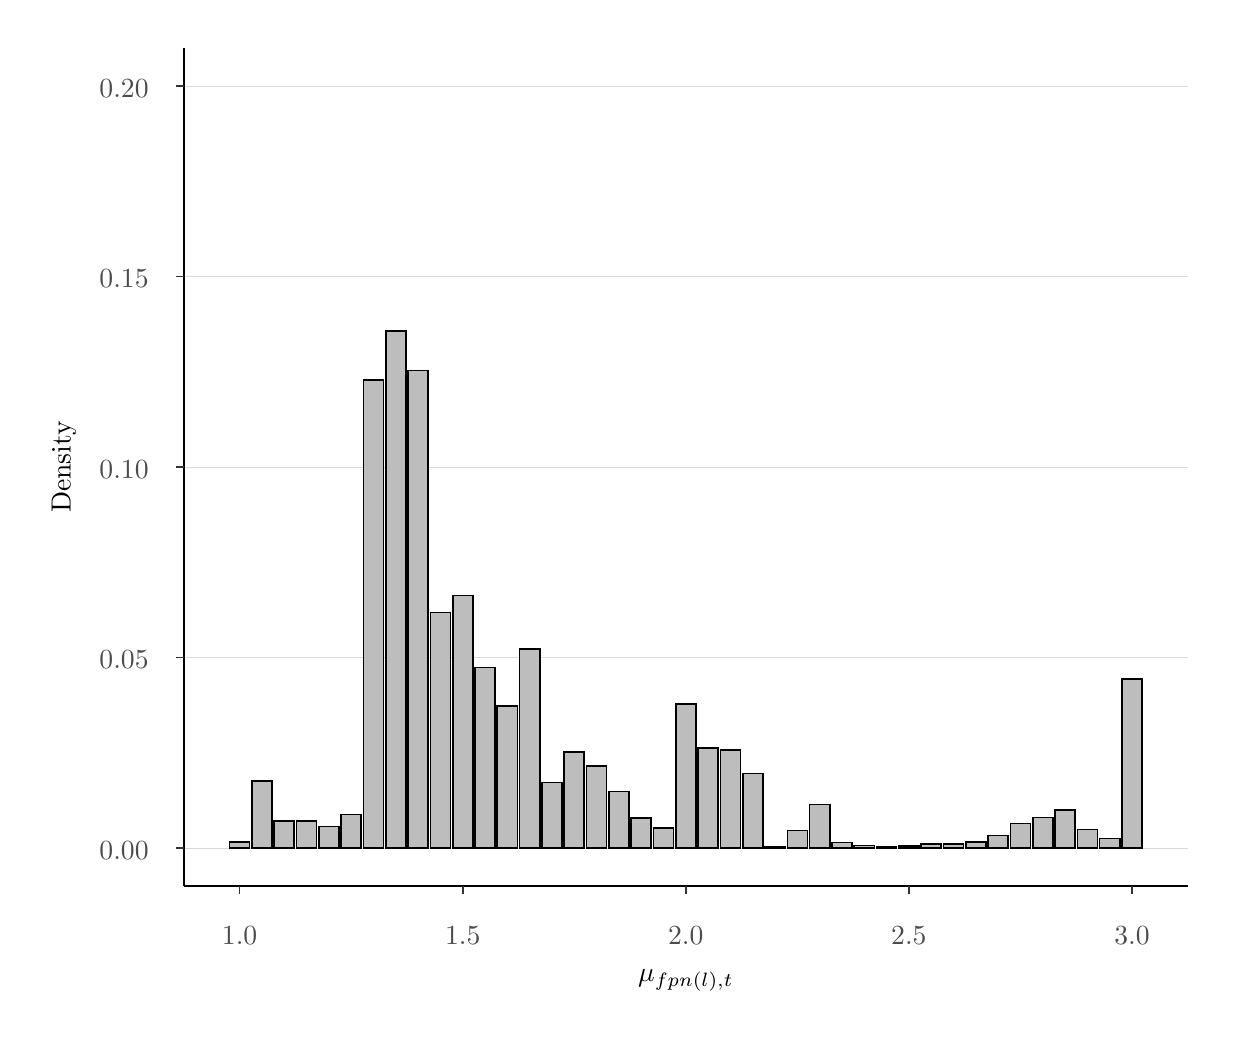
\begin{tikzpicture}[x=1pt,y=1pt]
\definecolor{fillColor}{RGB}{255,255,255}
\path[use as bounding box,fill=fillColor,fill opacity=0.00] (0,0) rectangle (433.62,361.35);
\begin{scope}
\path[clip] (  0.00,  0.00) rectangle (433.62,361.35);
\definecolor{drawColor}{RGB}{255,255,255}
\definecolor{fillColor}{RGB}{255,255,255}

\path[draw=drawColor,line width= 0.6pt,line join=round,line cap=round,fill=fillColor] ( -0.00,  0.00) rectangle (433.62,361.35);
\end{scope}
\begin{scope}
\path[clip] ( 56.47, 51.15) rectangle (419.17,354.12);
\definecolor{drawColor}{RGB}{255,255,255}

\path[draw=drawColor,line width= 0.3pt,line join=round] ( 56.47, 99.35) --
	(419.17, 99.35);

\path[draw=drawColor,line width= 0.3pt,line join=round] ( 56.47,168.21) --
	(419.17,168.21);

\path[draw=drawColor,line width= 0.3pt,line join=round] ( 56.47,237.07) --
	(419.17,237.07);

\path[draw=drawColor,line width= 0.3pt,line join=round] ( 56.47,305.92) --
	(419.17,305.92);

\path[draw=drawColor,line width= 0.3pt,line join=round] (116.89, 51.15) --
	(116.89,354.12);

\path[draw=drawColor,line width= 0.3pt,line join=round] (197.51, 51.15) --
	(197.51,354.12);

\path[draw=drawColor,line width= 0.3pt,line join=round] (278.12, 51.15) --
	(278.12,354.12);

\path[draw=drawColor,line width= 0.3pt,line join=round] (358.74, 51.15) --
	(358.74,354.12);
\definecolor{drawColor}{gray}{0.85}

\path[draw=drawColor,line width= 0.1pt,line join=round] ( 56.47, 64.92) --
	(419.17, 64.92);

\path[draw=drawColor,line width= 0.1pt,line join=round] ( 56.47,133.78) --
	(419.17,133.78);

\path[draw=drawColor,line width= 0.1pt,line join=round] ( 56.47,202.64) --
	(419.17,202.64);

\path[draw=drawColor,line width= 0.1pt,line join=round] ( 56.47,271.49) --
	(419.17,271.49);

\path[draw=drawColor,line width= 0.1pt,line join=round] ( 56.47,340.35) --
	(419.17,340.35);
\definecolor{drawColor}{RGB}{0,0,0}
\definecolor{fillColor}{gray}{0.74}

\path[draw=drawColor,line width= 0.6pt,line cap=rect,fill=fillColor] ( 72.95, 64.92) rectangle ( 80.21, 67.13);

\path[draw=drawColor,line width= 0.6pt,line cap=rect,fill=fillColor] ( 81.01, 64.92) rectangle ( 88.27, 89.09);

\path[draw=drawColor,line width= 0.6pt,line cap=rect,fill=fillColor] ( 89.08, 64.92) rectangle ( 96.33, 74.76);

\path[draw=drawColor,line width= 0.6pt,line cap=rect,fill=fillColor] ( 97.14, 64.92) rectangle (104.39, 74.76);

\path[draw=drawColor,line width= 0.6pt,line cap=rect,fill=fillColor] (105.20, 64.92) rectangle (112.45, 72.65);

\path[draw=drawColor,line width= 0.6pt,line cap=rect,fill=fillColor] (113.26, 64.92) rectangle (120.52, 77.04);

\path[draw=drawColor,line width= 0.6pt,line cap=rect,fill=fillColor] (121.32, 64.92) rectangle (128.58,234.00);

\path[draw=drawColor,line width= 0.6pt,line cap=rect,fill=fillColor] (129.38, 64.92) rectangle (136.64,251.84);

\path[draw=drawColor,line width= 0.6pt,line cap=rect,fill=fillColor] (137.45, 64.92) rectangle (144.70,237.44);

\path[draw=drawColor,line width= 0.6pt,line cap=rect,fill=fillColor] (145.51, 64.92) rectangle (152.76,149.99);

\path[draw=drawColor,line width= 0.6pt,line cap=rect,fill=fillColor] (153.57, 64.92) rectangle (160.83,156.13);

\path[draw=drawColor,line width= 0.6pt,line cap=rect,fill=fillColor] (161.63, 64.92) rectangle (168.89,130.18);

\path[draw=drawColor,line width= 0.6pt,line cap=rect,fill=fillColor] (169.69, 64.92) rectangle (176.95,116.13);

\path[draw=drawColor,line width= 0.6pt,line cap=rect,fill=fillColor] (177.76, 64.92) rectangle (185.01,136.78);

\path[draw=drawColor,line width= 0.6pt,line cap=rect,fill=fillColor] (185.82, 64.92) rectangle (193.07, 88.57);

\path[draw=drawColor,line width= 0.6pt,line cap=rect,fill=fillColor] (193.88, 64.92) rectangle (201.13, 99.71);

\path[draw=drawColor,line width= 0.6pt,line cap=rect,fill=fillColor] (201.94, 64.92) rectangle (209.20, 94.55);

\path[draw=drawColor,line width= 0.6pt,line cap=rect,fill=fillColor] (210.00, 64.92) rectangle (217.26, 85.33);

\path[draw=drawColor,line width= 0.6pt,line cap=rect,fill=fillColor] (218.06, 64.92) rectangle (225.32, 75.81);

\path[draw=drawColor,line width= 0.6pt,line cap=rect,fill=fillColor] (226.13, 64.92) rectangle (233.38, 72.23);

\path[draw=drawColor,line width= 0.6pt,line cap=rect,fill=fillColor] (234.19, 64.92) rectangle (241.44,117.04);

\path[draw=drawColor,line width= 0.6pt,line cap=rect,fill=fillColor] (242.25, 64.92) rectangle (249.51,101.06);

\path[draw=drawColor,line width= 0.6pt,line cap=rect,fill=fillColor] (250.31, 64.92) rectangle (257.57,100.38);

\path[draw=drawColor,line width= 0.6pt,line cap=rect,fill=fillColor] (258.37, 64.92) rectangle (265.63, 91.84);

\path[draw=drawColor,line width= 0.6pt,line cap=rect,fill=fillColor] (266.44, 64.92) rectangle (273.69, 65.42);

\path[draw=drawColor,line width= 0.6pt,line cap=rect,fill=fillColor] (274.50, 64.92) rectangle (281.75, 71.24);

\path[draw=drawColor,line width= 0.6pt,line cap=rect,fill=fillColor] (282.56, 64.92) rectangle (289.81, 80.67);

\path[draw=drawColor,line width= 0.6pt,line cap=rect,fill=fillColor] (290.62, 64.92) rectangle (297.88, 66.91);

\path[draw=drawColor,line width= 0.6pt,line cap=rect,fill=fillColor] (298.68, 64.92) rectangle (305.94, 65.83);

\path[draw=drawColor,line width= 0.6pt,line cap=rect,fill=fillColor] (306.74, 64.92) rectangle (314.00, 65.52);

\path[draw=drawColor,line width= 0.6pt,line cap=rect,fill=fillColor] (314.81, 64.92) rectangle (322.06, 65.67);

\path[draw=drawColor,line width= 0.6pt,line cap=rect,fill=fillColor] (322.87, 64.92) rectangle (330.12, 66.29);

\path[draw=drawColor,line width= 0.6pt,line cap=rect,fill=fillColor] (330.93, 64.92) rectangle (338.19, 66.31);

\path[draw=drawColor,line width= 0.6pt,line cap=rect,fill=fillColor] (338.99, 64.92) rectangle (346.25, 66.98);

\path[draw=drawColor,line width= 0.6pt,line cap=rect,fill=fillColor] (347.05, 64.92) rectangle (354.31, 69.44);

\path[draw=drawColor,line width= 0.6pt,line cap=rect,fill=fillColor] (355.12, 64.92) rectangle (362.37, 73.74);

\path[draw=drawColor,line width= 0.6pt,line cap=rect,fill=fillColor] (363.18, 64.92) rectangle (370.43, 76.00);

\path[draw=drawColor,line width= 0.6pt,line cap=rect,fill=fillColor] (371.24, 64.92) rectangle (378.49, 78.66);

\path[draw=drawColor,line width= 0.6pt,line cap=rect,fill=fillColor] (379.30, 64.92) rectangle (386.56, 71.62);

\path[draw=drawColor,line width= 0.6pt,line cap=rect,fill=fillColor] (387.36, 64.92) rectangle (394.62, 68.37);

\path[draw=drawColor,line width= 0.6pt,line cap=rect,fill=fillColor] (395.42, 64.92) rectangle (402.68,125.96);
\end{scope}
\begin{scope}
\path[clip] (  0.00,  0.00) rectangle (433.62,361.35);
\definecolor{drawColor}{RGB}{0,0,0}

\path[draw=drawColor,line width= 0.6pt,line join=round] ( 56.47, 51.15) --
	( 56.47,354.12);
\end{scope}
\begin{scope}
\path[clip] (  0.00,  0.00) rectangle (433.62,361.35);
\definecolor{drawColor}{gray}{0.30}

\node[text=drawColor,anchor=base east,inner sep=0pt, outer sep=0pt, scale=  1.00] at ( 43.72, 60.79) {0.00};

\node[text=drawColor,anchor=base east,inner sep=0pt, outer sep=0pt, scale=  1.00] at ( 43.72,129.65) {0.05};

\node[text=drawColor,anchor=base east,inner sep=0pt, outer sep=0pt, scale=  1.00] at ( 43.72,198.51) {0.10};

\node[text=drawColor,anchor=base east,inner sep=0pt, outer sep=0pt, scale=  1.00] at ( 43.72,267.36) {0.15};

\node[text=drawColor,anchor=base east,inner sep=0pt, outer sep=0pt, scale=  1.00] at ( 43.72,336.22) {0.20};
\end{scope}
\begin{scope}
\path[clip] (  0.00,  0.00) rectangle (433.62,361.35);
\definecolor{drawColor}{gray}{0.20}

\path[draw=drawColor,line width= 0.6pt,line join=round] ( 53.72, 64.92) --
	( 56.47, 64.92);

\path[draw=drawColor,line width= 0.6pt,line join=round] ( 53.72,133.78) --
	( 56.47,133.78);

\path[draw=drawColor,line width= 0.6pt,line join=round] ( 53.72,202.64) --
	( 56.47,202.64);

\path[draw=drawColor,line width= 0.6pt,line join=round] ( 53.72,271.49) --
	( 56.47,271.49);

\path[draw=drawColor,line width= 0.6pt,line join=round] ( 53.72,340.35) --
	( 56.47,340.35);
\end{scope}
\begin{scope}
\path[clip] (  0.00,  0.00) rectangle (433.62,361.35);
\definecolor{drawColor}{RGB}{0,0,0}

\path[draw=drawColor,line width= 0.6pt,line join=round] ( 56.47, 51.15) --
	(419.17, 51.15);
\end{scope}
\begin{scope}
\path[clip] (  0.00,  0.00) rectangle (433.62,361.35);
\definecolor{drawColor}{gray}{0.20}

\path[draw=drawColor,line width= 0.6pt,line join=round] ( 76.58, 48.40) --
	( 76.58, 51.15);

\path[draw=drawColor,line width= 0.6pt,line join=round] (157.20, 48.40) --
	(157.20, 51.15);

\path[draw=drawColor,line width= 0.6pt,line join=round] (237.82, 48.40) --
	(237.82, 51.15);

\path[draw=drawColor,line width= 0.6pt,line join=round] (318.43, 48.40) --
	(318.43, 51.15);

\path[draw=drawColor,line width= 0.6pt,line join=round] (399.05, 48.40) --
	(399.05, 51.15);
\end{scope}
\begin{scope}
\path[clip] (  0.00,  0.00) rectangle (433.62,361.35);
\definecolor{drawColor}{gray}{0.30}

\node[text=drawColor,anchor=base,inner sep=0pt, outer sep=0pt, scale=  1.00] at ( 76.58, 30.14) {1.0};

\node[text=drawColor,anchor=base,inner sep=0pt, outer sep=0pt, scale=  1.00] at (157.20, 30.14) {1.5};

\node[text=drawColor,anchor=base,inner sep=0pt, outer sep=0pt, scale=  1.00] at (237.82, 30.14) {2.0};

\node[text=drawColor,anchor=base,inner sep=0pt, outer sep=0pt, scale=  1.00] at (318.43, 30.14) {2.5};

\node[text=drawColor,anchor=base,inner sep=0pt, outer sep=0pt, scale=  1.00] at (399.05, 30.14) {3.0};
\end{scope}
\begin{scope}
\path[clip] (  0.00,  0.00) rectangle (433.62,361.35);
\definecolor{drawColor}{RGB}{0,0,0}

\node[text=drawColor,anchor=base,inner sep=0pt, outer sep=0pt, scale=  1.00] at (237.82, 16.79) {$\mu_{fpn(l),t}$};
\end{scope}
\begin{scope}
\path[clip] (  0.00,  0.00) rectangle (433.62,361.35);
\definecolor{drawColor}{RGB}{0,0,0}

\node[text=drawColor,rotate= 90.00,anchor=base,inner sep=0pt, outer sep=0pt, scale=  1.00] at ( 15.49,202.64) {Density};
\end{scope}
\end{tikzpicture}

     \parbox{\textwidth}{
        \begin{spacing}{1} 
            {\footnotesize 
            \textit{Notes}: This figure plots the distribution of firm-level markups. To account for the sampling variation in the elasticities of substitution, we bootstrap the markup distribution. In practice, we draw from the limiting distribution of the firm-level elasticities of substitution and for each bootstrap sample, we compute firm-level markups at the product category-firm-country-year level. Hereafter, we bin the absolute markup estimates into 40 separate bins and compute for each bin the number of observations that fall into each bin. Finally, we winsorize the markup distribution at a markup of 3.}
        \end{spacing}}
 \end{figure} 


\subsection{Regional Cost-of-living Differences}
We construct regional cost-of-living differences by computing each product category-region pair-year cell the log cost-of-living differences according to Equation \ref{eq:cle_decomp2}. To obtain a measure of variation in regional cost-of-living differences, we take the variance of log cost-of-living differences across product categories for each region pair-year. Table \ref{tab: var_decomp_cle} shows the mean and 95\% bootstrapped interval of the estimated variance of cost-of-living differences for intranational and international region pairs separately.\footnote{Bootstrapped confidence intervals are obtained by drawing blocks of households within regions with replacement and computing the cost-of-living differences for each of 100 bootstrap samples. To account for estimation in the elasticities of substitution, sampling and design-based uncertainty, we construct block-bootstrapped confidence intervals. In practice, we first draw region pairs with replacement and within each region pair, we draw a sample of consumers with replacement as well. Then, we draw firm- and product variety-level elasticities of substitution from their respective empirical distributions. Finally, for each bootstrap sample, we compute the overall cost-of-living differences, the different margins and their contribution.} Table \ref{tab: var_decomp_cle} also provides the mean and 95\% bootstrapped intervals of the three structural components presented in equation \ref{eq:cle_decomp2}. To construct each of these components, we rely on Equation \ref{eq:cle_decomp} and note that log cost-of-living differences can be written as the sum of three structural components. Therefore, the variance can be written as the sum of the variances of three terms and the covariances between them. As there is ex-ante no reason to favor any of the three terms, we then decompose the overall variance into these three terms by allocating the covariance terms equally.\footnote{\citet{Hottman2016} decomposes differences in sales or sales growth across firms into structural components by successive OLS estimations of the component on total sales. By doing so, the variance decomposition distributes the covariance terms equally across the different components.}.

First, consistent with the reduced-form evidence, cost-of-living differences for international pairs are larger compared to intranational pairs. On average, cost-of-living differences are eight times larger for intranational region pairs. While cost-of-living differences for international region pairs have a more dispersed distribution compared to international region pairs, it is mostly a shift in the conditional mean that drives the elevated cost-of-living differences. Nevertheless, even within countries, cost-of-living differences exist which is consistent with the results reported in \citet{Handbury2015} and in \citet{Feenstra2020} for the USA and China respectively. Second, decomposing cost-of-living differences into the three structural components provides more insight into the relevant margins for cost-of-living differences. For instance, pure taste differences have large explanatory power for regional cost-of-living differences. On average, they account for roughly 95\% and 64\% of the variation in cost-of-living differences for intranational and international region pairs respectively. This underscores the importance of filtering out taste differences when assessing the presence of geographic market segmentation. LOP deviations and choice set differences are relatively small for intranational region pairs but choice set differences matter much more for international pairs. A little over 40\% of the variation in regional cost-of-living differences across intranational region pairs is driven by choice set differences.  
 
\begin{table}
    \centering
    \caption{Variance decomposition of Cost-of-living differences}
    \label{tab: var_decomp_cle}
    \begin{spacing}{1.1}
        \scalebox{0.9}{
        \begin{tabular}{lcccc} 
            \toprule  
            $y_{ll',t}$ & $\text{CLE}_{ll',t}$ & $\text{LOP}_{ll',t}$ & $\text{Taste}_{ll',t}$ & $\text{Choice}_{ll',t}$  \\
            \cmidrule(lr){2-2} \cmidrule(lr){3-5} 
            & (1) & (2) & (3) & (4) \\ \midrule
            \multicolumn{5}{l}{\textsc{Panel A}: Intranational pairs ($B_{l'l} = 0$)} \\
            \myinput tables/estimation/P1_3_4_3_NCES_vardecomp_intra.tex \\ \midrule
            \multicolumn{5}{l}{\textsc{Panel B}: International pairs ($B_{l'l} = 1$)} \\
            \myinput tables/estimation/P1_3_4_3_NCES_vardecomp_inter.tex \\ \bottomrule
        \end{tabular}}
        \end{spacing}
    \vspace{5pt}
    \parbox{\textwidth}{
    \begin{spacing}{1} 
        {\footnotesize 
         \textit{Notes}: This table presents the overall variance and decomposition of log cost-of-living differences for intranational region pairs and international region pairs separately. Column (1) shows the average log cost-of-living difference for intranational region pairs in Panel A and for international region pairs in panel B. Below the estimate of the average log cost-of-living difference we display the 5\%-95\% confidence interval. We compute these statistics in four steps. First, within each bootstrap sample, we compute log cost-of-living differences following the expression displayed in Equation \ref{eq:cle_decomp}. Second, within each bootstrap sample, we compute the variance of log cost-of-living differences across product categories within each region pair-year cell. Third, within each bootstrap sample, we compute the average cost-of-living difference by averaging across region pair-year cells. Finally, the $\hat{\mathbb{E}}\left[\hat{\mathbb{V}}_{ll',t}\left(y_{pl'l,t}\right)\right]$ represents the average across bootstrap samples and the 5\%-95\% confidence intervals are $5^{\text{th}}$ and $95^{\text{th}}$ percentiles of the distribution across bootstrap samples. Columns (3) - columns (8) present the decomposition of the variance of log cost-of-living differences into the different margins. To compute the variance of each of the margins, we run the variance operator through the log-linear expression for log cost-of-living differences and allocate the covariance terms equally across each of the margins. In turn, we compute the average and the 5\%-95\% confidence interval for each of the components in the same way. For each margin, we also provide an estimate and a confidence interval of the share that each margin explains in the overall variance of log cost-of-living differences. For each bootstrap sample and for each margin, we compute this share as the ratio of the variance of the margin, averaged across region pair-year cells, to the variance of overall cost-of-living differences, averaged across region pair-year cells as well. In this way, $\hat{\mathbb{E}}\left[\hat{\mathbb{V}}_{ll',t}\left(y_{pl'l,t}\right)\right]\bigg/\hat{\mathbb{E}}\left[\hat{\mathbb{V}}_{ll',t}\left(\text{ln}\left(\frac{P_{pl',t}}{P_{pl,t}}\right)\right)\right]$ presents the average of this ratio across bootstrap samples and the 5\%-95\% confidence intervals are $5^{\text{th}}$ and $95^{\text{th}}$ percentiles of the distribution of this share across bootstrap samples.}
    \end{spacing}}
\end{table}